\chapter{Estudo de Caso}
\label{sec:estudo_de_caso}
Para a condução do estudo de caso da aplicação, com ênfase na identificação dos pontos de incremento de produtividade, o \textit{framework} Laravel foi selecionado como referência para comparação. Esta escolha se fundamenta em sua ampla disseminação, especialmente entre os \textit{frameworks} que satisfazem os critérios estabelecidos para comparação neste trabalho, a saber: ser direcionado ao desenvolvimento \textit{web}, possuir uma arquitetura claramente definida e oferecer suporte à utilização de um ORM, seja de forma nativa ou preparado para receber um ORM externo. Como ilustração, uma base de dados foi empregada como exemplificação, contendo relacionamentos entre entidades, a saber, usuários (\textit{users}), empresas (\textit{teams}) e postagens (\textit{posts}), representado pela figura . Destaca-se que a relação entre usuários e postagens foi estabelecida mediante o emprego de uma tabela intermediária. Uma representação visual das tabelas que constituem esta base de dados é apresentada na Figura~\ref{fig:enter-label}.

\begin{figure}[H]
    \centering
    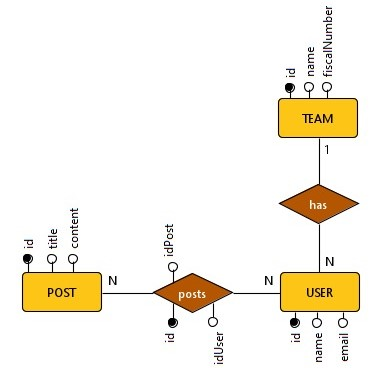
\includegraphics[width=0.6\linewidth]{figures/caso_de_uso_der.jpeg}
    \caption{Estudo de caso construído usando o GenDBM Tool~\citep{alexandre23}.}
    \label{fig:enter-label}
\end{figure}

Para ilustrar dois cenários potenciais, inicialmente considerando a premissa de que a base de dados já tenha sido estabelecida, o que pode ocorrer em projetos migrados de outras tecnologias ou ser a preferência de desenvolvedores que optam pela criação direta no gerenciador de banco de dados, procederemos à execução do comando responsável pela engenharia reversa da base de dados. Esse comando tem por finalidade traduzir a estrutura da base de dados em classes de migrações, as quais possibilitam o versionamento das tabelas e afins da aplicação no que tange a base de dados relacional. Dessa maneira, ao empregar um comando específico, é factível obter uma economia de tempo e recursos, cujo alcance é exponencialmente proporcional à complexidade da base de dados. Abaixo está o comando executado e o resultado das migrações geradas relativo a base de dados determinada para o estudo de caso.

\spaceH{}
\lstinputlisting[language=bash,caption=Comando para engenharia reversa da base de dados]{scripts/cosmo_db_reverse.bash}

\spaceH{}
\lstinputlisting[language=bash,caption=Exemplo criação de rotas]{scripts/db_reverse_example_result.php}
\label{scripts/db_reverse_example_result.php}

Em situações em que projetos são concebidos a partir do zero, essas classes necessitam ser construídas manualmente, um procedimento análogo ao adotado no contexto do Laravel. Progredindo para a etapa subsequente, relativo à representação das entidades por meio de classes modelo e seus respectivos relacionamentos, os quais são gerenciados e interpretados pelo ORM, tanto no ambiente do Vortex quanto no Laravel. No caso do Vortex, é possível empregar o comando de tradução, o qual realiza de maneira automática o mapeamento citado. Em contraste, no Laravel, não está disponível uma tecnologia equivalente de mapeamento automático de modelos e relacionamentos. Tal processo de mapeamento proporciona uma economia significativa de tempo e conhecimento, com impacto proporcional ao número de entidades relacionais, particularmente quando comparado a um projeto no Laravel, onde a criação manual de todos os modelos e relacionamentos é imperativa. Abaixo é exibido o exemplo do resultado da utilização deste comando com as entidades deste caso de uso.

\spaceH{}
\lstinputlisting[language=php,caption=Comando para tradução automatica das entidades relacionais em modelos]{scripts/db_translate_result_example.php}
\label{scripts/db_translate_result_example.php}

\subsection{Ambiente}
Para demostrar a comparação de performance foram gerados dados em ambiente controlado tanto temporal quanto em questão de \textit{hardware}, para garantir uma melhor veracidade dos dados, sendo realizado em uma máquina contendo:

\begin{itemize}
    \item Processador - AMD Ryzen 5 7535HS.
    \item Memória RAM - 8 \textit{gigabytes} DDR5 4800 MHz.
    \item Sistema operacional - Windows 10 PRO.
    \item Armazenamento - 512 GB SSD NVMe PCIe 4.0.
    \item PHP - 8.2.0
    \item SGBD - MySQL 8.0.0
\end{itemize}

Cada teste foi realizado em \textit{loops} de cem repetições ou de mil repetições, este último para processos mais rápidos. Cada teste foi adaptado para cada estrutura de cada um dos \textit{frameworks} mais difundidos no contexto deste trabalho. Para não haver influências terceiras de outras funcionalidades, foi utilizada uma série de abstrações feitas em PHP nativo sem quaisquer resquício de ferramentas dos \textit{frameworks} para realizar o teste, à exceção do \textit{script} sujeito à análise. Os testes foram realizados em uma base de dados contendo as seguintes quantidades de registros:

\begin{itemize}
    \item Tabela de usuários - 1000.
    \item Tabela de postagens - 10000.
    \item Tabela de empresas - 100.
    \item Tabela relacionando usuários e postagens - 100000.
\end{itemize}
\section{Experimentos}
Para realização de testes voltados para performance focando nos ORMs em diversos tipos de consultas e interações com a base de dados, baseou-se no parâmetro de tempo de processamento como medida de comparação. As conexões realizadas com a base de dados não representam diferenças expressivas, a grande diferença está no ORM e na hora de converter dados em objetos modelo mapeados juntamente com seus relacionamentos. Algumas decisões de desenvolvimento em relação aos ORMs podem torna-los custosos e lentos, por parte do Laravel destacam-se o uso de \textit{reflections}, citadas em \ref{rt_reflections}, que degradam a performance além de decisões pontuais como para buscar relacionamentos realizar duas consultas, uma para buscar os identificadores do modelo principal e outra para buscar os relacionamentos. As operações de conexão efetuadas com a base de dados não revelam disparidades significativas; entretanto, a distinção preponderante manifesta-se no desempenho dos ORMs e na fase de conversão de dados em objetos modelo, incluindo seus respectivos relacionamentos.
\subsection{Resultados}
Os cenários para teste foram: seleção completa da tabela de usuários (\textit{SELECT *}), seleção do primeiro usuário (\textit{SELECT FIRST}), seleção do último usuário (\textit{SELECT LAST}), criação e deleção de um usuário (\textit{CREATE AND DELETE}), seleção condicional de um usuário (\textit{SELECT WHERE}) e seleção ordenada de usuários (\textit{SELECT ORDER}). Os resultados desses testes, abarcando uma variedade de contextos pertinentes à utilização de ORMs, são apresentados a seguir.

\begin{figure}[H]
    \centering
    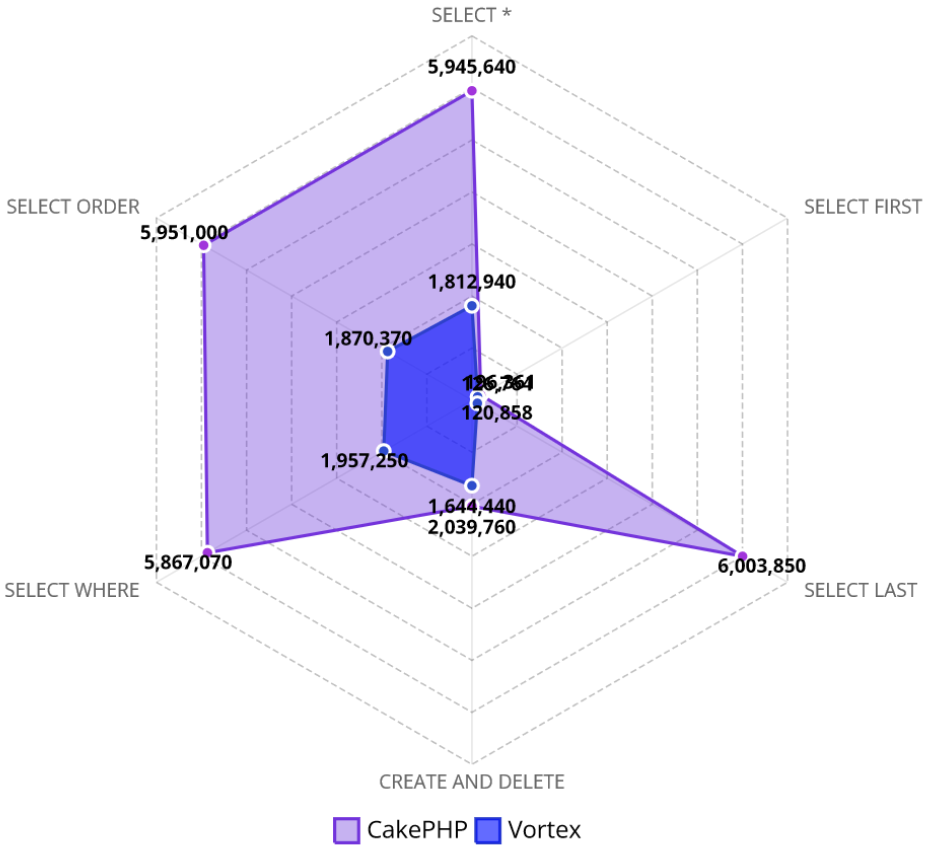
\includegraphics[width=0.7\linewidth]{figures/vortex_vs_cakephp.png}
    \caption{Gráfico comparativo performance ORM CakePHP e Vortex}
    \label{fig:vortex_vs_cakephp}
\end{figure}

\begin{table}[H] \footnotesize
\fontsize{9pt}{9pt}\selectfont
\centering
\vspace{1cm}
\begin{tabular}{|c|c|c|c|}
\hline  
& Vortex & CakePHP & CakePHP / Vortex\\
\hline 
SELECT * & 1812940 ns & 5945640 ns & $\approx$ 3,279x \\
SELECT FIRST & 126764 ns  & 196361 ns & $\approx$ 1,549x \\
SELECT LAST & 120858 ns  & 6003850 ns & $\approx$ 49,676x \\
CREATE AND DELETE & 1644440 ns & 2039760 ns & $\approx$ 1,240x \\
SELECT WHERE & 1957250 ns & 5867070 ns & $\approx$ 2,997x \\
SELECT ORDER & 1870370 ns & 5951000 ns & $\approx$ 3,181x \\
\hline
\end{tabular}
\caption{Proporcionalidade na performance entre \textit{frameworks}: análise do número de vezes em que o Vortex supera o CakePHP em testes controlados}
\label{vortex_vs_cakephp}
\end{table}

\begin{figure}[H]
    \centering
    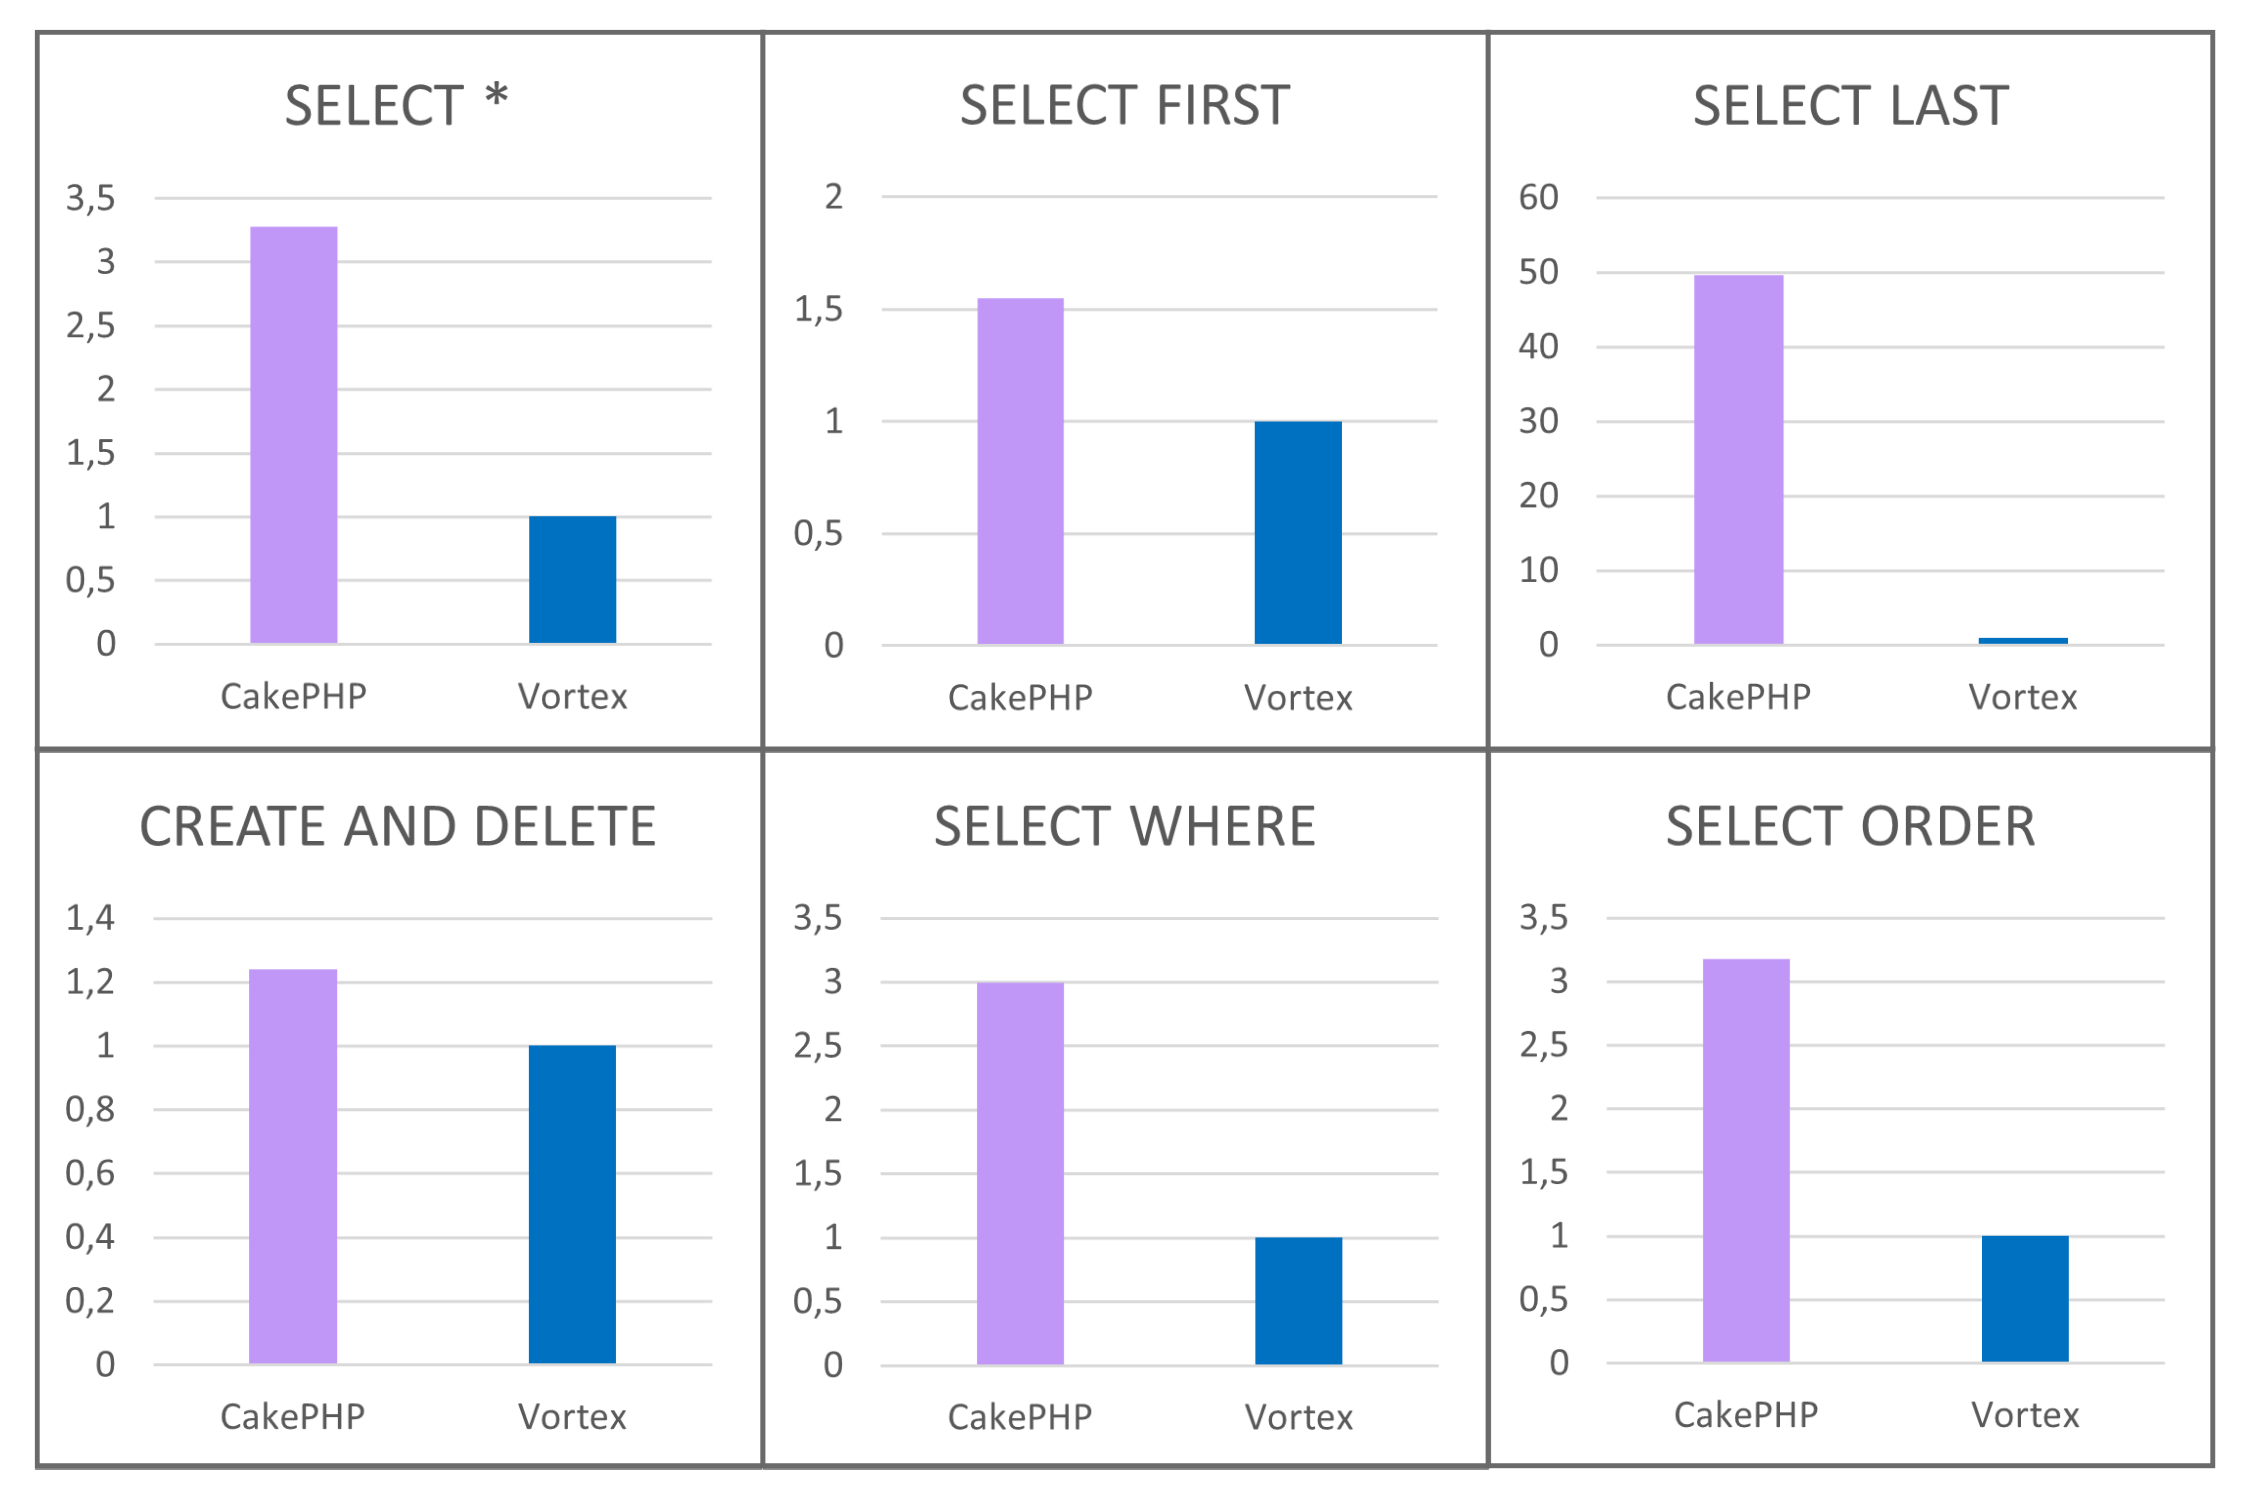
\includegraphics[width=0.9\linewidth]{figures/vortex_vs_cakephp_barcode.png}
    \caption{Gráfico comparativo performance ORM CakePHP e Vortex}
    \label{fig:vortex_vs_cakephp_barcode}
\end{figure}

A análise dos dados gerados mediante a comparação entre o CakePHP e o Vortex, conforme ilustrado nas Figuras \ref{fig:vortex_vs_cakephp},  \ref{fig:vortex_vs_cakephp_barcode}, bem como sumarizado na Tabela \ref{vortex_vs_cakephp}, revela as seguintes constatações:

\begin{enumerate}
    \item Na execução da consulta completa utilizando a cláusula \textit{SELECT *}, observou-se que o CakePHP manifestou um desempenho aproximadamente $\approx$ 3,279 vezes mais custoso. 
    \item Ao direcionar a consulta para recuperar o primeiro registro  \textit{SELECT FIRST}, constatou-se que o CakePHP apresentou um custo aproximado de $\approx$ 1,549 vezes superior em relação ao Vortex. 
    \item A realização da consulta para obter o último registro \textit{SELECT LAST} revelou um desproporcional incremento no tempo de execução pelo CakePHP, alcançando um custo aproximadamente $\approx$ 49,676 vezes maior em comparação ao Vortex.
    \item No contexto da criação e deleção de um usuário \textit{CREATE AND DELETE}, constatou-se que o CakePHP implicou em um custo aproximado de $\approx$ 1,240 vezes superior.
    \item Nas consultas condicionais \textit{SELECT WHERE}, o CakePHP apresentou um custo aproximadamente $\approx$ 2,997 vezes mais elevado.
    \item Em consultas ordenadas \textit{SELECT ORDER}, verificou-se que o CakePHP registrou um custo aproximadamente $\approx$ 3,181 vezes superior em comparação ao Vortex.
\end{enumerate}

\begin{figure}[H]
    \centering
    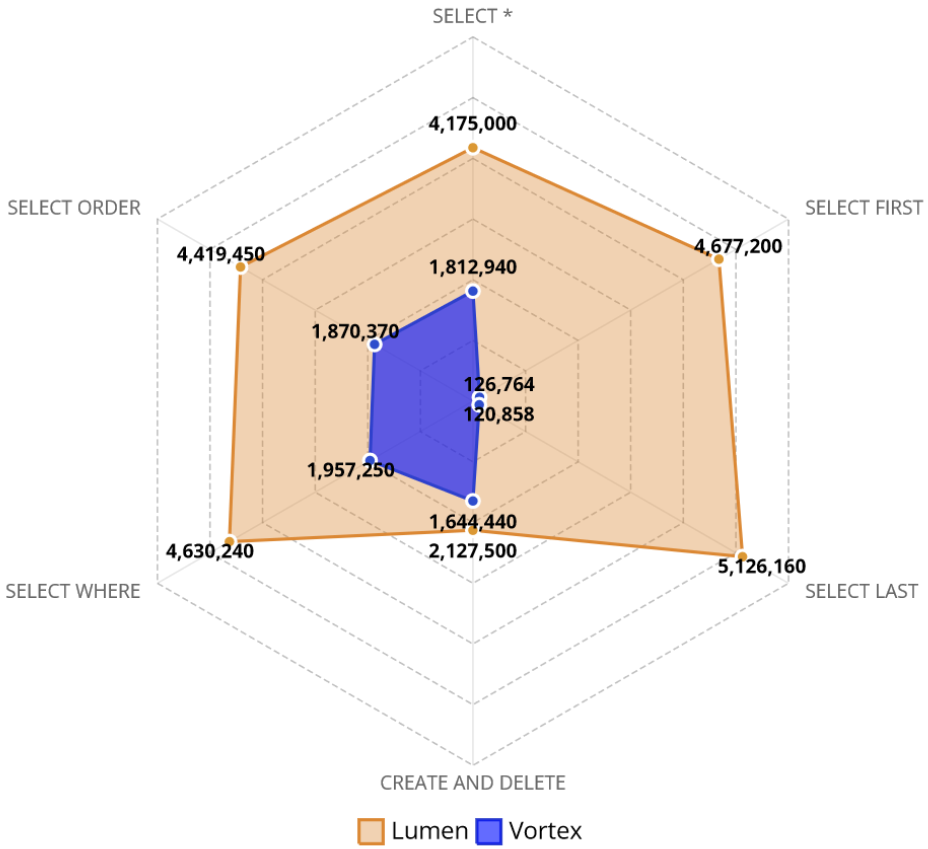
\includegraphics[width=0.7\linewidth]{figures/vortex_vs_lumen.png}
    \caption{Gráfico comparativo performance ORM Lumen e Vortex}
    \label{fig:vortex_vs_lumen}
\end{figure}

\begin{table}[H] \footnotesize
\fontsize{9pt}{9pt}\selectfont
\centering
\vspace{1cm}
\begin{tabular}{|c|c|c|c|}
\hline  
& Vortex & Lumen & Lumen / Vortex\\
\hline 
SELECT * & 1812940 ns & 4175000 ns & $\approx$ 2,302x \\
SELECT FIRST & 126764 ns  & 4677200 ns & $\approx$ 36,896x \\
SELECT LAST & 120858 ns  & 5126160 ns & $\approx$ 42,414x \\
CREATE AND DELETE & 1644440 ns & 2127500 ns & $\approx$ 1,293x \\
SELECT WHERE & 1957250 ns & 4630240 ns & $\approx$ 2,365x \\
SELECT ORDER & 1870370 ns & 4419450 ns & $\approx$ 2,362x \\
\hline
\end{tabular}
\caption{Proporcionalidade na performance entre \textit{frameworks}: análise do número de vezes em que o Vortex supera o Lumen em testes controlados}
\label{vortex_vs_lumen}
\end{table}

\begin{figure}[H]
    \centering
    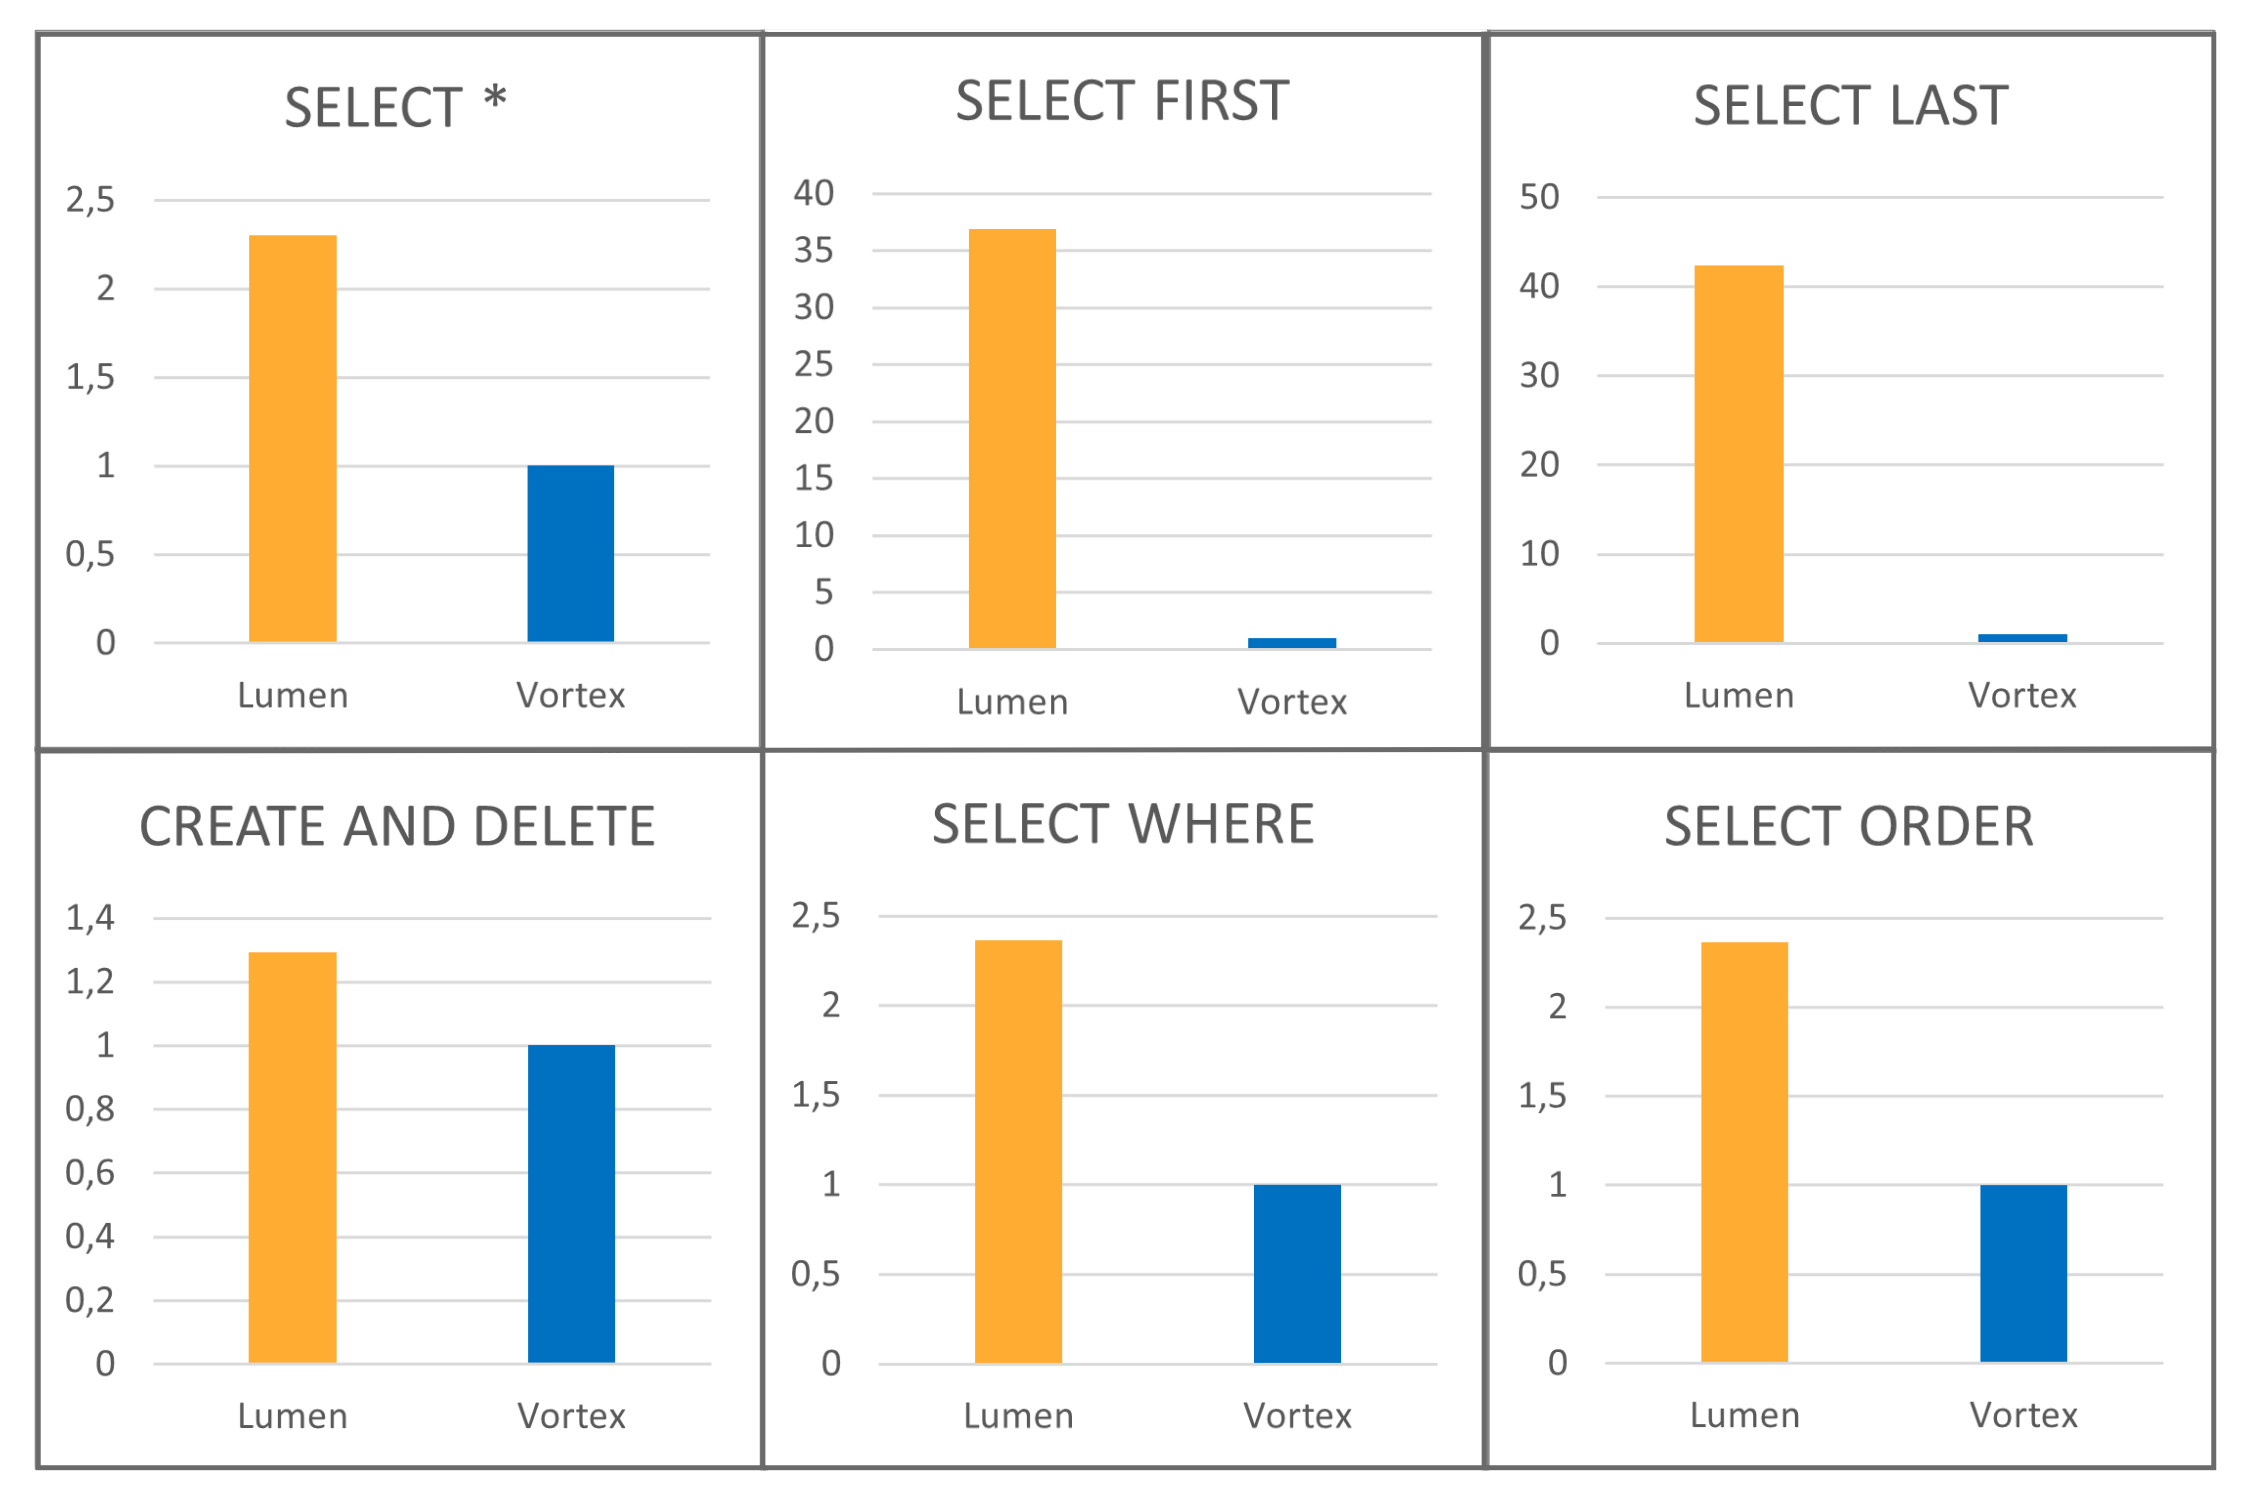
\includegraphics[width=0.9\linewidth]{figures/vortex_vs_lumen_barcode.png}
    \caption{Gráfico comparativo performance ORM Lumen e Vortex}
    \label{fig:vortex_vs_lume_barcode}
\end{figure}

A análise dos dados obtidos por meio da comparação entre o Lumen e o Vortex, conforme evidenciado nas Figuras \ref{fig:vortex_vs_lumen} e \ref{fig:vortex_vs_lume_barcode}, e devidamente sumarizado na Tabela \ref{vortex_vs_lumen}, proporciona revelações significativas:

\begin{enumerate}
    \item No contexto da execução da consulta completa utilizando a cláusula \textit{SELECT *}, observou-se que o Lumen demonstrou um desempenho aproximadamente $\approx$ 2,302 vezes mais dispendioso.
    \item Ao direcionar a consulta para recuperar o primeiro registro (\textit{SELECT FIRST}), verificou-se que o Lumen implicou em um custo aproximado de $\approx$ 36,896 vezes superior em relação ao Vortex.
    \item A condução da consulta para obtenção do último registro (\textit{SELECT LAST}) revelou um notável incremento no tempo de execução pelo Lumen, alcançando um custo aproximadamente $\approx$ 42,414 vezes maior em comparação ao Vortex.
    \item No âmbito da criação e exclusão de um usuário (\textit{CREATE AND DELETE}), constatou-se que o Lumen acarretou um custo aproximado de $\approx$ 1,293 vezes superior.
    \item Nas consultas condicionais (\textit{SELECT WHERE}), o Lumen demonstrou um custo aproximadamente $\approx$ 2,365 vezes mais elevado.
    \item Em consultas ordenadas (\textit{SELECT ORDER}), observou-se que o Lumen registrou um custo aproximadamente $\approx$ 2,362 vezes superior em comparação ao Vortex.
\end{enumerate}

\begin{figure}[H]
    \centering
    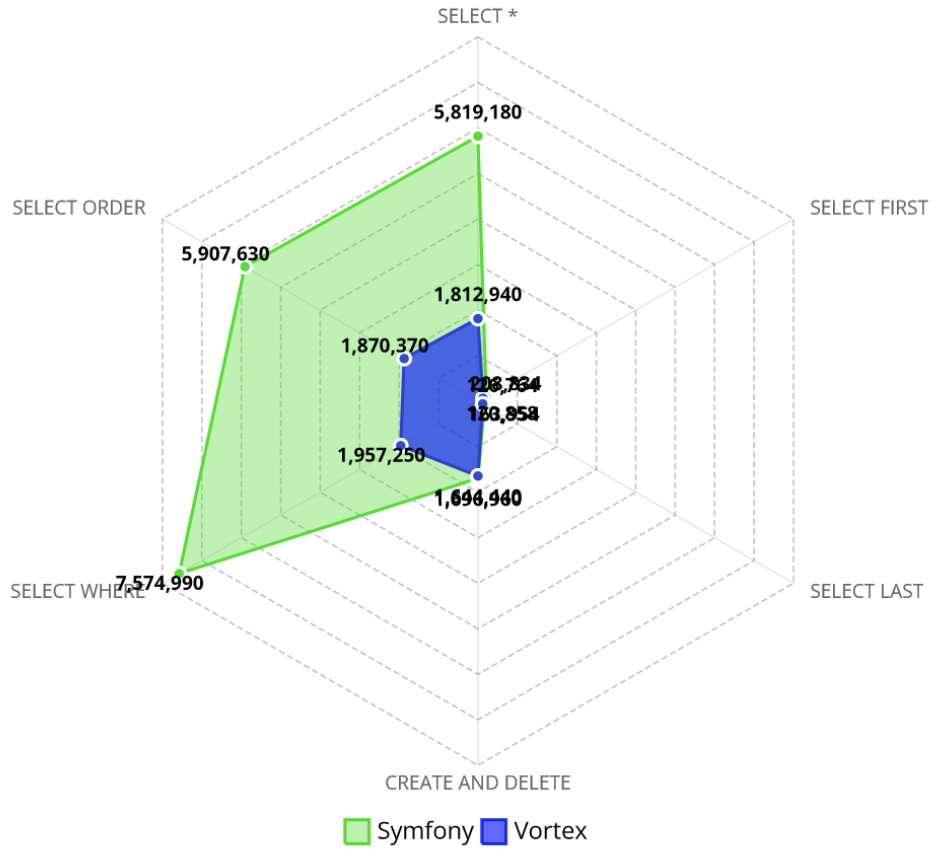
\includegraphics[width=0.7\linewidth]{figures/vortex_vs_symfony.png}
    \caption{Gráfico comparativo performance ORM Symfony e Vortex}
    \label{fig:vortex_vs_symfony}
\end{figure}

\begin{table}[H] \footnotesize
\fontsize{9pt}{9pt}\selectfont
\centering
\vspace{1cm}
\begin{tabular}{|c|c|c|c|}
\hline  
& Vortex & Symfony & Symfony / Vortex\\
\hline 
SELECT * & 1812940 ns & 5819180 ns & $\approx$ 3,209x \\
SELECT FIRST & 126764 ns  & 208834 ns & $\approx$ 1,647x \\
SELECT LAST & 120858 ns  & 163954 ns & $\approx$ 1,356x \\
CREATE AND DELETE & 1644440 ns & 1696960 ns & $\approx$ 1,031x \\
SELECT WHERE & 1957250 ns & 7574990 ns & $\approx$ 3,870x \\
SELECT ORDER & 1870370 ns & 5907630 ns & $\approx$ 3,158x \\
\hline
\end{tabular}
\caption{Proporcionalidade na performance entre \textit{frameworks}: análise do número de vezes em que o Vortex supera o Symfony em testes controlados}
\label{vortex_vs_symfony}
\end{table}

\begin{figure}[H]
    \centering
    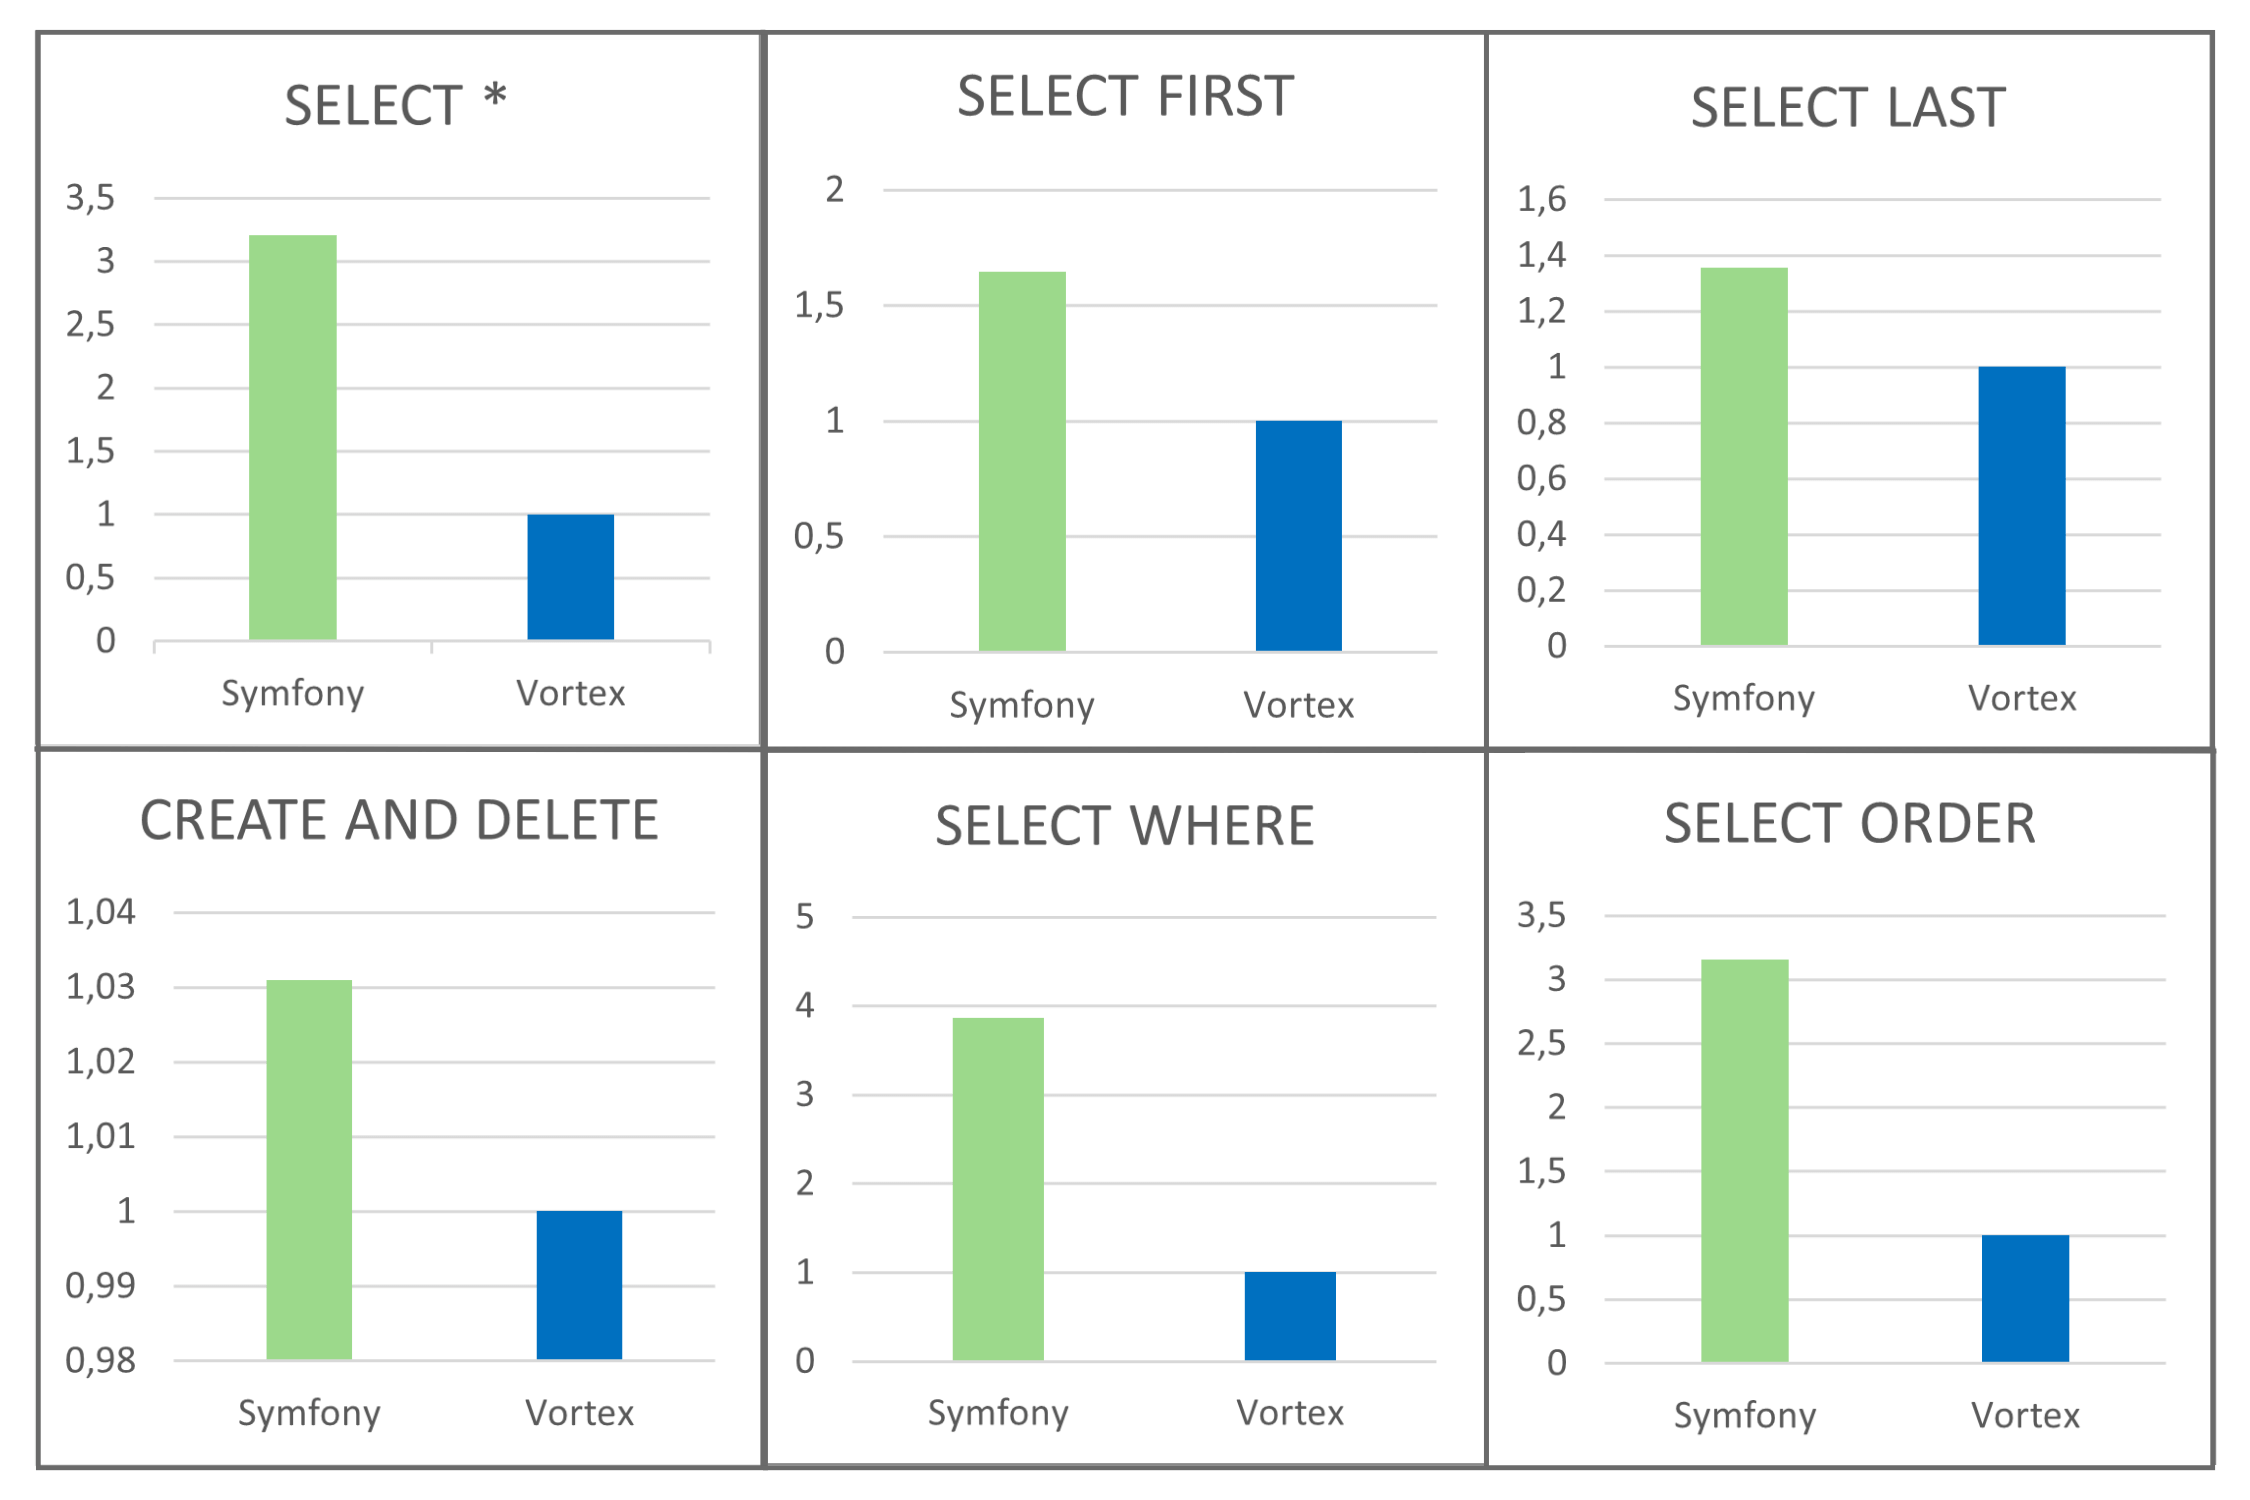
\includegraphics[width=0.9\linewidth]{figures/vortex_vs_symfony_barcode.png}
    \caption{Gráfico comparativo performance ORM Symfony e Vortex}
    \label{fig:vortex_vs_symfony_barcode}
\end{figure}

A análise dos dados decorrentes da comparação entre o Symfony e o Vortex, conforme ilustrado nas Figuras \ref{fig:vortex_vs_symfony} e \ref{fig:vortex_vs_symfony_barcode}, e devidamente resumido na Tabela \ref{vortex_vs_symfony}, proporciona importantes conclusões:

\begin{enumerate}
    \item No contexto da realização da consulta completa utilizando a cláusula \textit{SELECT *}, constatou-se que o \textit{framework} Symfony exibiu um desempenho aproximadamente $\approx$ 3,209 vezes mais oneroso.
    \item Ao focalizar a consulta para recuperar o primeiro registro (\textit{SELECT FIRST}), verificou-se que o Symfony implicou em um custo aproximado de $\approx$ 1,647 vezes superior em relação ao Vortex.
    \item A condução da consulta para obtenção do último registro (\textit{SELECT LAST}) revelou um notável incremento no tempo de execução pelo Symfony, alcançando um custo aproximadamente $\approx$ 1,356 vezes maior em comparação ao Vortex.
    \item No escopo da criação e exclusão de um usuário (\textit{CREATE AND DELETE}), constatou-se que o Symfony acarretou um custo aproximado de $\approx$ 1,031 vezes superior.
    \item Nas consultas condicionais (\textit{SELECT WHERE}), o Symfony manifestou um custo aproximadamente $\approx$ 3,870 vezes mais elevado.
    \item Em consultas ordenadas (\textit{SELECT ORDER}), observou-se que o Symfony registrou um custo aproximadamente $\approx$ 3,158 vezes superior em comparação ao Vortex.
\end{enumerate}


\begin{figure}[H]
    \centering
    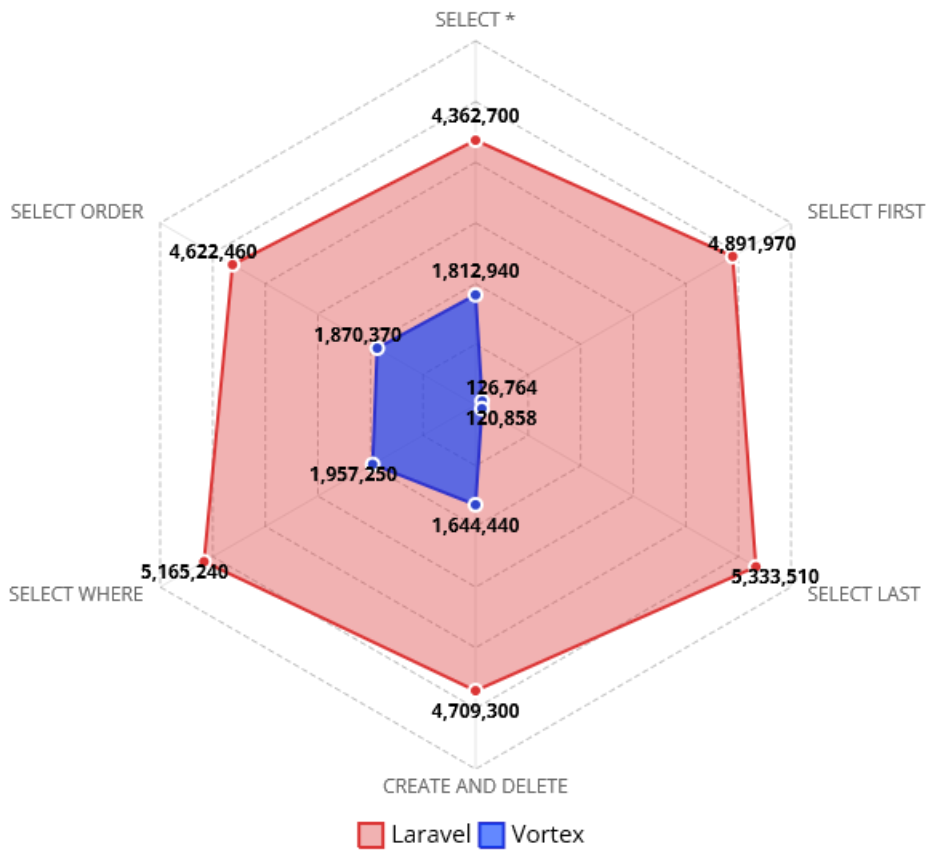
\includegraphics[width=0.7\linewidth]{figures/vortex_vs_laravel.png}
    \caption{Gráfico comparativo performance ORM Laravel e Vortex}
    \label{fig:vortex_vs_laravel}
\end{figure}

\begin{table}[H] \footnotesize
\fontsize{9pt}{9pt}\selectfont
\centering
\vspace{1cm}
\begin{tabular}{|c|c|c|c|}
\hline  
& Vortex & Laravel & Laravel / Vortex\\
\hline 
SELECT * & 1812940 ns & 4362700 ns & $\approx$ 2,406x \\
SELECT FIRST & 126764 ns  & 4891970 ns & $\approx$ 38,591x \\
SELECT LAST & 120858 ns  & 5333510 ns & $\approx$ 44,130x \\
CREATE AND DELETE & 1644440 ns & 4709300 ns & $\approx$ 2,863x \\
SELECT WHERE & 1957250 ns & 5165240 ns & $\approx$ 2,639x \\
SELECT ORDER & 1870370 ns & 4622460 ns & $\approx$ 2,471x \\
\hline
\end{tabular}
\caption{Proporcionalidade na performance entre \textit{frameworks}: análise do número de vezes em que o Vortex supera o Laravel em testes controlados}
\label{vortex_vs_laravel}
\end{table}

\begin{figure}[H]
    \centering
    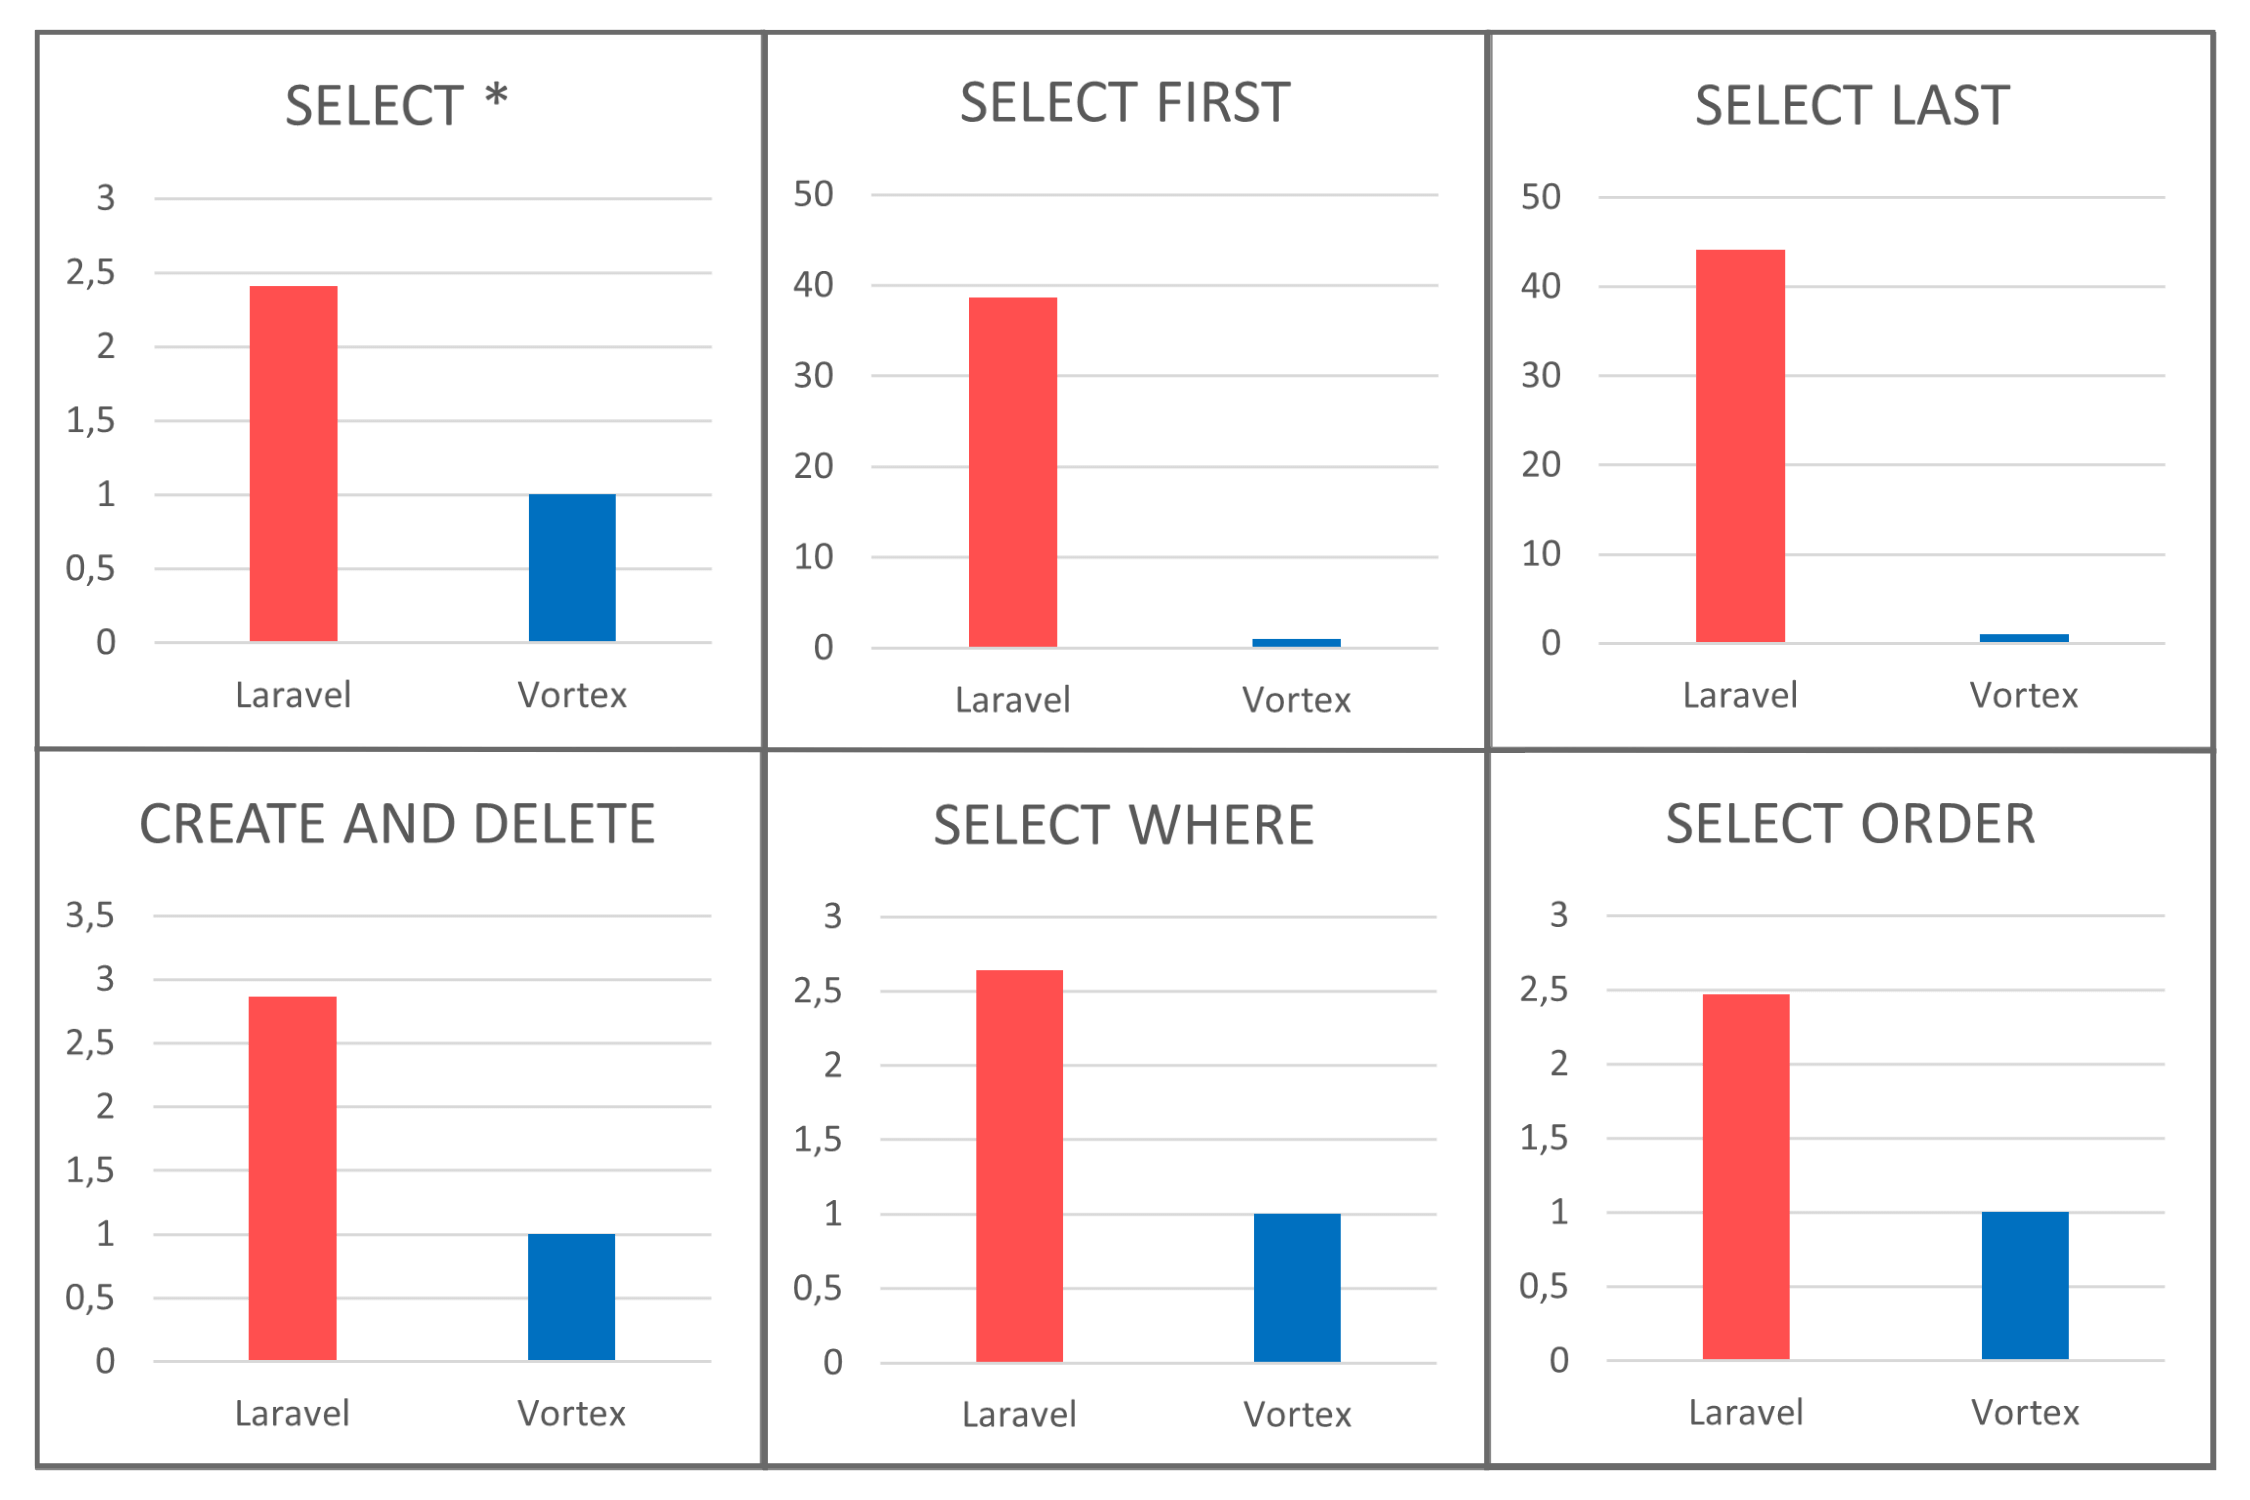
\includegraphics[width=0.9\linewidth]{figures/vortex_vs_laravel_barcode.png}
    \caption{Gráfico comparativo performance ORM Laravel e Vortex}
    \label{fig:vortex_vs_laravel_barcode}
\end{figure}

A avaliação dos dados resultantes da comparação entre o Laravel e o Vortex, conforme representado nas Figuras \ref{fig:vortex_vs_laravel} e \ref{fig:vortex_vs_laravel_barcode}, e devidamente resumida na Tabela \ref{vortex_vs_laravel}, conduz as seguintes conclusões:

\begin{enumerate}
    \item Na execução da pesquisa completa usando a cláusula \textit{SELECT *}, foi observado que o \textit{framework} Laravel demonstrou um desempenho aproximadamente $\approx$ 2,406 vezes mais dispendioso.
    \item Ao direcionar a consulta para recuperar o primeiro registro (\textit{SELECT FIRST}), verificou-se que o Laravel resultou em um custo aproximado de $\approx$ 38,591 vezes superior em relação ao Vortex.
    \item A realização da consulta para obtenção do último registro (\textit{SELECT LAST}) evidenciou um significativo aumento no tempo de execução pelo Laravel, resultando em um custo aproximadamente $\approx$ 44,130 vezes maior em comparação ao Vortex.
    \item No âmbito da criação e exclusão de um usuário (\textit{CREATE AND DELETE}), constatou-se que o Laravel gerou um custo aproximado de $\approx$ 2,863 vezes superior.
    \item Nas consultas condicionais (\textit{SELECT WHERE}), o Laravel revelou um custo aproximadamente $\approx$ 2,639 vezes mais elevado.
    \item Em consultas ordenadas (\textit{SELECT ORDER}), foi observado que o Laravel registrou um custo aproximadamente $\approx$ 2,471 vezes superior em comparação ao Vortex.
\end{enumerate}

De maneira isolada, procedemos à análise das consultas envolvendo relacionamentos, representadas através do uso da cláusula \textit{SELECT WITH}. No âmbito deste estudo, tais consultas se referem à obtenção de informações sobre usuários e suas respectivas relações de postagens, consolidadas em uma única instrução de consulta executada pelo Mapeador Objeto-Relacional (ORM). Adicionalmente, foram examinadas as consultas denominadas \textit{CALL RELATIONS}, as quais têm como objetivo recuperar exclusivamente os valores pertinentes a um relacionamento específico, desconsiderando a entidade primária que deu origem a tal relacionamento, neste caso, os usuários. As Figuras \ref{fig:call_relations} e \ref{fig:select_with} apresentam os resultados obtidos em virtude da execução destas modalidades de consulta. As tabelas \ref{call_relations_table} e \ref{select_with_table} apresentam os dados usados pelos gráficos citados.

\begin{figure}[H]
    \centering
    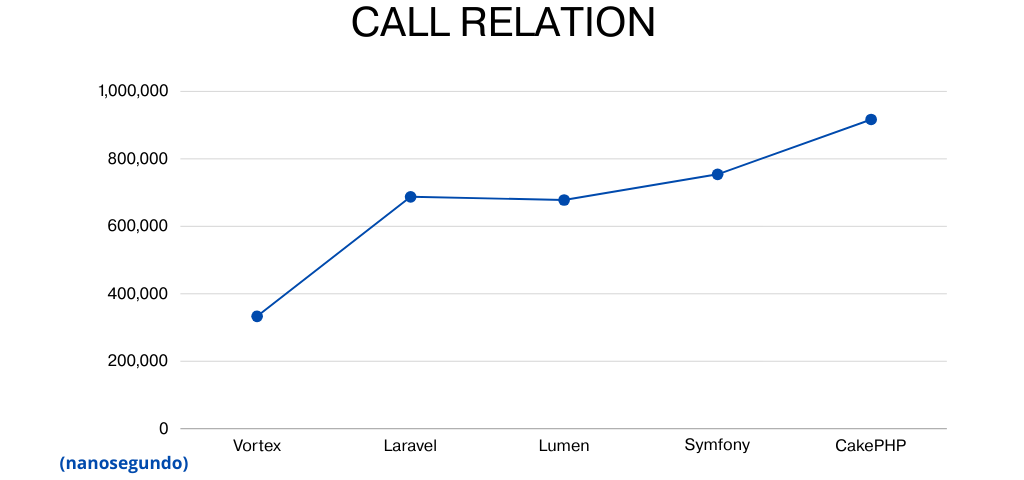
\includegraphics[width=0.9\linewidth]{figures/call_relations.png}
    \caption{Gráfico comparativo performance ORM dos \textit{frameworks} em relacionamentos}
    \label{fig:call_relations}
\end{figure}

\begin{table}[H] \footnotesize
\fontsize{9pt}{9pt}\selectfont
\centering
\vspace{1cm}
\begin{tabular}{|c|c|c|c|}
\hline
Framework & Tempo de Execução(ns)\\
\hline 
Vortex  & 333283 ns \\
Laravel & 687478 ns \\
Lumen   & 678044 ns \\
Symfony & 754170 ns \\
CakePHP & 916754 ns \\
\hline
\end{tabular}
\caption{Tempo de execução consultas de relacionamentos entre os \textit{frameworks}}
\label{call_relations_table}
\end{table}

\begin{figure}[H]
    \centering
    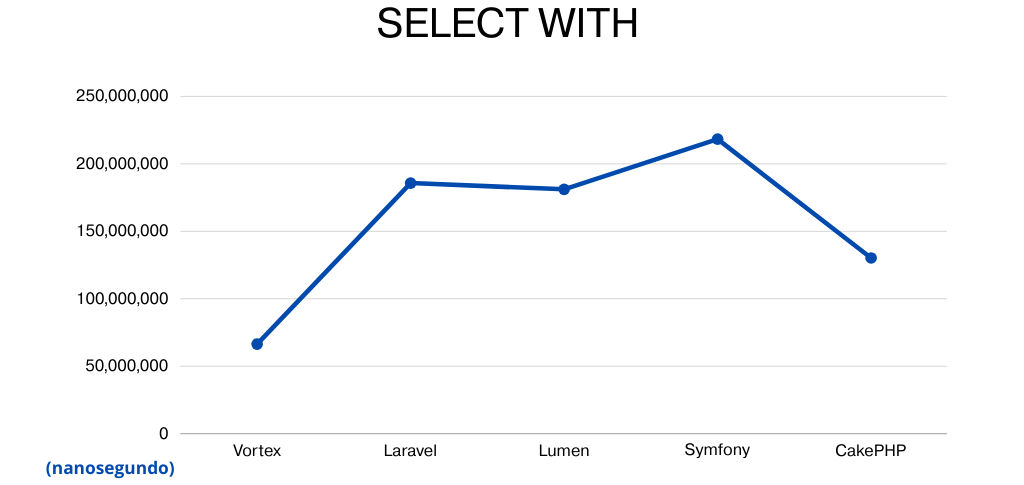
\includegraphics[width=0.9\linewidth]{figures/select_with.png}
    \caption{Gráfico comparativo performance ORM dos \textit{frameworks} em relacionamentos carregados na entidade primaria}
    \label{fig:select_with}
\end{figure}

\begin{table}[H] \footnotesize
\fontsize{9pt}{9pt}\selectfont
\centering
\vspace{1cm}
\begin{tabular}{|c|c|c|c|}
\hline
Framework & Tempo de Execução(ns)\\
\hline 
Vortex  & 66426900 ns \\
Laravel & 185758000 ns \\
Lumen   & 181123000 ns \\
Symfony & 218312000 ns \\
CakePHP & 130254000 ns \\
\hline
\end{tabular}
\caption{Tempo de execução entre os \textit{frameworks} em consultas de entidades carregando relacionamentos}
\label{select_with_table}
\end{table}

Com base nos dados expostos nas tabelas, é possível inferir que, em ambas as consultas, observou-se uma superioridade do Vortex em comparação aos demais \textit{frameworks}. No contexto da Tabela \ref{call_relations_table}, na consulta denominada \textit{CALL RELATION}, registrou-se o menor tempo de execução após a utilização do Vortex, sendo o Lumen aquele que apresentou aproximadamente $\approx$ 2,034 vezes o tempo de execução do Vortex. Por outro lado, o CakePHP evidenciou o desempenho menos favorável, apresentando um tempo de execução aproximadamente $\approx$ 2,750 vezes superior ao do Vortex. Já em consultas \textit{SELECT WITH} também se observa a vantagem do Vortex em relação ados demais \textit{frameworks}, sendo novamente o pior comparado foi o Symfony com 218312000 ns e aproximadamente $\approx$ 3,286 vezes mais lento que o Vortex. Já o melhor comparado ao Vortex foi o Lumen com 181123000 ns e $\approx$ 2,726 vezes o tempo de execução do Vortex.

Os resultados dos testes práticos são ilustrados nas figuras: \ref{fig:vortex_vs_cakephp}, \ref{fig:vortex_vs_lumen}, \ref{fig:vortex_vs_symfony}, \ref{fig:vortex_vs_laravel}, \ref{fig:call_relations} e \ref{fig:select_with}, evidenciando a superioridade de desempenho do Vortex em comparação com outros \textit{frameworks}. Com o mesmo propósito de avaliação dos parâmetros de performance, a análise se concentra no tempo de execução de rotinas específicas em cada \textit{framework}, focalizando a comparação entre Vortex e Laravel. Os dados apresentados nas tabelas \ref{vortex_vs_laravel} são confrontados em termos de nanossegundos, sendo que a última coluna à direita representa a razão relativa ao tempo de execução do Laravel em relação ao Vortex. Dessa maneira, é possível observar quantas vezes as rotinas do Laravel demandaram mais tempo do que as correspondentes no Vortex. Já as consultas de relacionamentos mostraram vantagem para o Vortex em relação ao Laravel na ordem de $\approx$ 2,062 para o cenário de \textit{CALL RELATION} e para \textit{SELECT WITH} $\approx$ 2,796.
